\documentclass[titlepage, fleqn, a4paper, 12pt, twoside]{article}
\usepackage{geometry}
\usepackage{exsheets} %question and solution environments
\usepackage{amsmath, amssymb, amsthm} %standard AMS packages
\usepackage[utf8]{inputenc}
\usepackage{esint} %integral signs
\usepackage{marginnote} %marginnotes
\usepackage{gensymb} %miscellaneous symbols
\usepackage{commath} %differential symbols
\usepackage{xcolor} %colours
\usepackage{cancel} %cancelling terms
\usepackage[free-standing-units,space-before-unit]{siunitx} %formatting units
	\sisetup
	{
		per-mode=fraction,
		fraction-function=\frac
	}
\usepackage{tikz, pgfplots} %diagrams
	\usetikzlibrary{calc, hobby, patterns, intersections, angles, quotes, spy}
	\usetikzlibrary{circuits.logic.US,circuits.logic.IEC}
\usepackage{graphicx} %inserting graphics
\usepackage{imakeidx}
\makeindex
\usepackage{hyperref} %hyperlinks
\usepackage{datetime} %date and time
\usepackage{enumerate, enumitem} %numbered lists
\usepackage{float} %inserting floats
\usepackage[american voltages]{circuitikz} %circuit diagrams
\usepackage{setspace} %double spacing
\usepackage{microtype} %micro-typography
\usepackage{listings} %formatting code
	\lstset{language=Matlab}
	\lstdefinestyle{standardMatlab}
	{
		belowcaptionskip=1\baselineskip,
		breaklines=true,
		frame=L,
		xleftmargin=\parindent,
		language=C,
		showstringspaces=false,
		basicstyle=\footnotesize\ttfamily,
		keywordstyle=\bfseries\color{green!40!black},
		commentstyle=\itshape\color{purple!40!black},
		identifierstyle=\color{blue},
		stringstyle=\color{orange},
	}
\usepackage{booktabs}
\usepackage{multirow}
\usepackage{todonotes}
\usepackage[noabbrev,capitalize]{cleveref}
\usepackage[section]{placeins}
\usepackage[style=numeric, backend=biber]{biblatex}
\usepackage{adjustbox}
\usepackage{algpseudocode} %algorithms
\usepackage{algorithm} %algorithms

% \bibliography{<mybibfile>}% ONLY selects .bib file; syntax for version <= 1.1b
\addbibresource{bibliography.bib}% Syntax for version >= 1.2

\newcommand\numberthis{\addtocounter{equation}{1}\tag{\theequation}} %adds numbers to specific equations in non-numbered list of equations

\DeclareMathAlphabet{\mathcal}{OT1}{pzc}{m}{it}

\theoremstyle{definition}
\newtheorem{example}{Example}
\newtheorem{definition}{Definition}

\theoremstyle{theorem}
\newtheorem{theorem}{Theorem}
\newtheorem{law}{Law}

\tikzset{
block/.style = {draw, rectangle, minimum height=3em, minimum width=3em},
tmp/.style  = {coordinate},
sum/.style = {draw, circle, node distance=1cm},
input/.style = {coordinate},
output/.style = {coordinate},
pinstyle/.style = {pin edge={to-,thin,black}}
}

\makeatletter
\@addtoreset{section}{part} %resets section numbers in new part
\makeatother

\newcommand\blfootnote[1]{%
	\begingroup
	\renewcommand\thefootnote{}\footnote{#1}%
	\addtocounter{footnote}{-1}%
	\endgroup
}

\renewcommand{\marginfont}{\scriptsize \color{blue}}

\renewcommand{\tilde}{\widetilde}

\def\doubleunderline#1{\underline{\underline{#1}}}

\SetupExSheets{solution/print = true} %prints all solutions by default

\DeclareMathOperator{\FT}{\mathcal{FT}}
\DeclareMathOperator{\DTFT}{\mathcal{DTFT}}
\DeclareMathOperator{\IFT}{\mathcal{FT}^{-1}}
\DeclareMathOperator{\IDTFT}{\mathcal{DTFT}^{-1}}
\DeclareMathOperator{\DFT}{\mathcal{DFT}}
\DeclareMathOperator{\FFT}{\mathcal{FFT}}

\DeclareMathOperator{\Q}{\mathcal{Q}}

\DeclareMathOperator{\rect}{\mathrm{rect}}
\DeclareMathOperator{\sinc}{\mathrm{sinc}}

\DeclareMathOperator{\boxfunc}{\mathrm{box}}

\DeclareMathOperator{\vspan}{\mathrm{span}}

\DeclareMathOperator{\argmin}{\mathrm{argmin}}

\DeclareMathOperator{\Db}{\mathrm{Db}}

\DeclareMathOperator{\normal}{\mathrm{N}}

\DeclareMathOperator{\expct}{\mathrm{E}}

\DeclareMathOperator{\sgn}{\mathrm{sgn}}

\DeclareMathOperator{\dist}{\mathrm{d}}

\DeclareMathOperator{\nullspace}{\mathrm{N}}
\DeclareMathOperator{\range}{\mathrm{R}}

\DeclareMathOperator{\l2}{\ell_2}

\DeclareMathOperator{\rank}{\mathrm{rank}}
\DeclareMathOperator{\diag}{\mathrm{diag}}

\def\transpose#1{{#1}^{\mathsf{T}}}
\def\minustranspose#1{{#1}^{\mathsf{-T}}}

\def\downsample#1{\downarrow_{#1}}
\def\upsample#1{\uparrow_{#1}}

%opening
\title{Digital Processing of Single and Multidimensional Signals}
\author{Aakash Jog}
\date{2018-19}

\begin{document}

\pagenumbering{roman}
\begin{titlepage}
\newgeometry{margin=0cm}
\maketitle
\end{titlepage}
\restoregeometry
%\setlength{\mathindent}{0pt}

\blfootnote
{
	\begin{figure}[H]
		\includegraphics[height = 12pt]{cc.pdf}
		\includegraphics[height = 12pt]{by.pdf}
		\includegraphics[height = 12pt]{nc.pdf}
		\includegraphics[height = 12pt]{sa.pdf}
	\end{figure}
	This work is licensed under the Creative Commons Attribution-NonCommercial-ShareAlike 4.0 International License. To view a copy of this license, visit \url{http://creativecommons.org/licenses/by-nc-sa/4.0/}.
} %CC-BY-NC-SA license

\tableofcontents

\clearpage
\section{Lecturer Information}

\textbf{Dr. Raja Giryes}\\
~\\
E-mail: \href{mailto:raja@tauex.tau.ac.il}{raja@tauex.tau.ac.il}\\
~\\

\section{Grading}

\begin{enumerate}
	\item Homework (MATLAB or NumPy): 20\%
	\item Final exam: 80\%
\end{enumerate}

\clearpage
\pagenumbering{arabic}

\part{Basic Definition and Theorems}

\begin{definition}[Fourier transform]
	For an LTI system, the Fourier transform is defined as
	\begin{align*}
		\FT\left\{ x(t) \right\} &= \left\langle x,e^{2 \pi j f t} \right\rangle\\
		&= \int\limits_{t \in \mathrm{R}^d} x(t) \overline{e^{2 \pi j f t}} \dif t\\
		&= \int\limits_{t \in \mathrm{R}^d} x(t) e^{-2 \pi j \transpose{f} t} \dif t
	\end{align*}
	\label{def:Fourier_transform}
	\index{transform!Fourier!continuous time}
\end{definition}

\begin{definition}[Tensor product]
	\begin{align*}
		(x_1 \otimes \dots \otimes x_d)(t) &= x_1(t_1) \cdot \dots \cdot x_d(t_d)
	\end{align*}
	for $t \in R^d$.
	\index{product!tensor}
\end{definition}

\begin{definition}[Fourier transform of tensor product]
	The Fourier transform of a tensor product is defined as
	\begin{align*}
		\FT\left\{ x_1 \otimes \dots \otimes x_d \right\}(f) &= \int\limits_{R^d} x_1(t_1) \cdot \dots \cdot x_d(t_d) e^{-2 \pi j (t_1 f_1 + \dots + t_d f_d)} \dif t_1 \dots \dif t_d\\
		&= \left( \FT\left\{ x_1(t) \right\}(f_1) \right) \dots \left( \FT\left\{ x_d(t) \right\}(f_d) \right)
	\end{align*}
	\index{transform!Fourier!continuous time}
	\index{product!tensor}
\end{definition}

\begin{definition}[$\rect$]
	\begin{align*}
		\rect(t) &=
			\begin{cases}
				0 &;\quad |t| > \frac{1}{2}\\
				1 &;\quad |t| < \frac{1}{2}\\
			\end{cases}
	\end{align*}
	\index{standard functions!rect}
\end{definition}

\begin{definition}[$u_{[a,b]}$]
	\begin{align*}
		u_{[a,b]}(t) &=
			\begin{cases}
				1 &;\quad a \le t \le b\\
				0 &;\quad \text{otherwise}\\
			\end{cases}
	\end{align*}
	\index{standard functions!u@$u_{[a,b]}$}
\end{definition}

\begin{definition}[$\sinc$]
	\begin{align*}
		\sinc(t) &= \frac{\sin(\pi t)}{\pi t}
	\end{align*}
	\index{standard functions!sinc}
\end{definition}

\begin{theorem}
	\begin{align*}
		\FT\left\{ \rect(t) \right\} &= \sinc(f)
	\end{align*}
	\index{standard functions!rect}
	\index{standard functions!sinc}
\end{theorem}

\begin{definition}[$\boxfunc$]
	A box function is defined to be the product of rect functions in multiple dimensions.
	\begin{align*}
		\boxfunc(t_1,\dots,t_n) &= \rect(t_1) \cdot \dots \cdot \rect(t_n)\\
		&=
			\begin{cases}
				1 &;\quad |t_1| < \frac{1}{2}, \dots, |t_n| < \frac{1}{2}\\
				0 &;\quad \text{otherwise}\\
			\end{cases}
	\end{align*}
	\index{standard functions!box}
	\index{standard functions!rect}
\end{definition}

\begin{definition}[Signum function]
	The signum function is defined to be
	\begin{align*}
		\sgn(t) &=
			\begin{cases}
				1 &;\quad t > 0\\
				[-1,1] &;\quad t = 0\\
				-1 &;\quad t < 0\\
			\end{cases}
	\end{align*}
	\index{standard functions!sgn}
\end{definition}

\begin{theorem}[Shifting in time]
	\begin{align*}
		\FT\left\{ D_p\left( x(t) \right) \right\}(f) &= e^{-2 \pi j \transpose{f} p} \FT\left\{ x(t) \right\}(f)
	\end{align*}
	where
	\begin{align*}
		D_p\left( x(t) \right) &= x(t - p)
	\end{align*}
	\label{thm:shifting_in_time}
	\index{shift!in time}
\end{theorem}

\begin{theorem}
	\begin{align*}
		x(t) \ast h(t) &= \FT{x}(f) \FT{h}(f)
	\end{align*}
	\label{thm:convolution_in_time_multiplication_in_frequency}
	\index{convolution!in time}
	\index{multiplication!in frequency}
\end{theorem}

\begin{theorem}[Stretching in time]
	\begin{align*}
		\FT\left\{ S_A\left( x(t) \right) \right\}(f) &= \int\limits_{R^d} x(A t) e^{-j 2 \pi \transpose{f} t} \dif t\\
		&= \int\limits_{R^d} x(q) ^{-j 2 \pi \transpose{f} A^{-1} q} \frac{\dif q}{|\det A|}\\
		&= \frac{1}{|\det A|} \int\limits_{R^d}  x(q) e^{-j 2 \pi \left( \minustranspose{A} f \right)^T q} \dif q\\
		&= \frac{\FT\left\{ x(t) \right\}\left( \minustranspose{A} f \right)}{|\det A|}\\
		&= \frac{S_{\minustranspose{A}} X(f)}{|\det A|}
	\end{align*}
	where
	\begin{align*}
		S_A\left( x(t) \right) &= x(A t)
	\end{align*}
	where $A$ is a matrix which may represent stretching, rotating, etc.\\
	Hence, if $A$ is equal to a scalar $a$,
	\begin{align*}
		\FT\left\{ x(a t) \right\} &= \frac{\FT\left\{ x(t) \right\}\left( \frac{f}{a} \right)}{|a|}
	\end{align*}
	\label{thm:stretching_in_time}
	\index{stretch!in time}
\end{theorem}

\begin{theorem}[Fourier transform of Gaussian]
	Using \cref{thm:stretching_in_time}, for a single dimensional Gaussian signal,
	\begin{align*}
		\FT\left\{ e^{-t^2} \right\} &= e^{-\pi f^2}
	\end{align*}
	and for a orthogonal multidimensional Gaussian,
	\begin{align*}
		\FT\left\{ e^{-\transpose{t} t} \right\} &= e^{-\pi \transpose{f} f}
	\end{align*}
	Hence, using \cref{thm:stretching_in_time}, for a general multidimensional Gaussian,
	\begin{align*}
		\FT\left\{ e^{-\transpose{t} C^{-1} t} \right\} &= e^{-\pi \transpose{f} C f} |\det C|
	\end{align*}
	where $C$ is the covariance matrix.
	\label{thm:Fourier_transform_of_Gaussian}
	\index{transform!Fourier!continuous time}
	\index{standard functions!Gaussian}
\end{theorem}

\begin{definition}[Unitary matrix]
	A matrix $A$ is said to be unitary if
	\begin{align*}
		A^{-1} &= A^*
	\end{align*}
	where $A^*$ is the conjugate transpose of $A$.
	\index{types of matrices!unitary}
	\index{conjugate transpose}
\end{definition}

\begin{theorem}[Rotation]
	Stretching with by a unitary matrix $A$ is equivalent to rotation, and hence denoting $S_A$ by $R_R$,
	\begin{align*}
		\FT\left\{ R_R\left( x(t) \right) \right\} &= R_R \FT\left\{ x(t) \right\}
	\end{align*}
	\label{thm:rotation}
	\index{stretch!in time}
	\index{rotation!in time}
\end{theorem}

\begin{definition}
	A dimension-reducing projection $P$ from $R^d$ to $R^{d - 1}$, is defined as
	\begin{align*}
		P\left( x(t) \right) &= \int\limits_{R^d} x(t_1,\dots,t_d) \dif t_d
	\end{align*}
	\index{projection!dimension-reducing}
\end{definition}

\begin{definition}
	The slicing operator $\Q$ is defined as
	\begin{align*}
		\Q\left\{ X(f_1,\dots,f_d) \right\} &= X\left( f_1,\dots,f_{d - 1},0 \right)
	\end{align*}
	\label{def:slicing_operator}
	\index{standard operators!slicing}
\end{definition}

\begin{theorem}[Fourier transform of dimension reducing projection]
	The Fourier transform of a dimension reducing projection is
	\begin{align*}
		\FT\left\{ P\left( x(t) \right) \right\} &= \int\limits_{R^{d - 1}} \left( \int\limits_{R^d} x(t_1,\dots,t_d) \dif t_d \right) e^{-j 2 \pi (t_1 f_1 + \dots + t_{d - 1} f_{d - 1})} \dif t_1 \dots \dif t_{d - 1}\\
		&= \int\limits_{R^{d - 1}} \left( \int\limits_{R^d} x(t_1,\dots,t_d) e^{-j 2 \pi t_d (0)} \dif t_d \right) e^{-j 2 \pi (t_1 f_1 + \dots + t_{d - 1} f_{d - 1})} \dif t_1 \dots \dif t_{d - 1}\\
		&= \int\limits_{R^d} x(t) e^{-j 2 \pi \transpose{f} t} \dif t \Big|_{f_d = 0}\\
		&= \FT\left\{ x(t) \right\}(f_1,\dots,f_{d - 1},0)\\
		&= \Q\left\{ \FT\left\{ x(t) \right\} \right\}
	\end{align*}
	where $\Q$ is the slicing operator as in \cref{def:slicing_operator}.
	\label{thm:Fourier_transform_of_dimension_reducing_projection}
	\index{projection!dimension-reducing}
	\index{transform!Fourier!continuous time}
\end{theorem}

\clearpage
\part{Hilbert Spaces}

\section{Inner Product Spaces}

\begin{definition}[Inner product spaces]
	An inner product space is defined to be a space with an inner product with the following properties.
	\begin{description}
		\item[Conjugate symmetry]
			\begin{align*}
				\langle x,y \rangle &= \langle y,x \rangle^*
			\end{align*}
		\item[Linearity]
			\begin{align*}
				\langle x , a y + b z \rangle &= a \langle x,y \rangle + b \langle x,z \rangle
			\end{align*}
		\item[Non-negativity]
			\begin{equation*}
				\langle x,x \rangle = 0 \iff x = 0
			\end{equation*}
	\end{description}
	\index{spaces!inner product}
\end{definition}

\begin{definition}[Norm and distance]
	The norm corresponding to an inner product space is defined to be
	\begin{align*}
		\|x\| &= \sqrt{\langle x,x \rangle}
	\end{align*}
	Hence, the distance between $x$ and $y$ is defined to be
	\begin{align*}
		\dist(x,y) &= \|x - y\|
	\end{align*}
	\index{norm}
	\index{distance}
\end{definition}

\begin{definition}[Hilbert space]
	An inner product, normed, complete vector space is said to be a Hilbert space.
	\index{spaces!Hilbert}
\end{definition}

\section{Operators and Transformations}

\begin{theorem}
	Let $M$ be an operator from the inner product space $H$ to the inner product space $S$.
	Then,
	\begin{align*}
		\langle M x , y \rangle &= \langle x , M^* y \rangle
	\end{align*}
	for all $x \in H$ and $y \in S$.
	If $H$ and $S$ are finite, then $M$ can be represented by a matrix and
	\begin{align*}
		M^* &= \overline{M^T}
	\end{align*}
	is the complex transpose of $M$.
	\index{operators}
\end{theorem}

\begin{definition}[Linear operator]
	An operator $T$ is said to be linear if
	\begin{align*}
		T(a_1 x_1 + a_2 x_2) &= a_1 T(x_1) + a_2 T(x_2)
	\end{align*}
	\index{types of operators!linear}
\end{definition}

\begin{theorem}[Bounded linear operation]
	All linear operators are bounded, i.e. for every $T$, there exists $\alpha$ such that
	\begin{align*}
		\left\| T(x) \right\| &\le \alpha \|x\|
	\end{align*}
	for all $x$.
	\index{types of operators!linear}
\end{theorem}

\begin{theorem}[Continuous linear operation]
	If there exists a sequence $x_i$ which converges to $x$, then for any linear operator $T$, the sequence $T(x_i)$ converges to $T(x)$.
	\index{types of operators!linear}
\end{theorem}

\begin{definition}[Adjoint of linear operation]
	The adjoint of a linear operation $T$ is defined to be $T^*$, the only bounded operation such that
	\begin{align*}
		\langle T x , y \rangle &= \langle x , T^* y \rangle
	\end{align*}
	for all $x \in H$, $y \in S$.\\
	\index{adjoint of linear operation}
\end{definition}

\begin{definition}[Unitary operator]
	An operator $T$ is said to be unitary if and only if
	\begin{align*}
		T T^* &= T^* T\\
		&= I
	\end{align*}
	where $T^*$ is the conjugate transpose of $T$.
	\index{types of operators!unitary}
\end{definition}

\begin{definition}[Hermitian operator]
	An operator $T$ is said to be Hermitian if and only if
	\begin{align*}
		T^* &= T
	\end{align*}
	where $T^*$ is the conjugate transpose of $T$.
	\index{types of operators!Hermitian}
\end{definition}

\begin{theorem}
	An operator $T$ from a Hilbert space $H$ to $H$ is Hermitian if and only if
	\begin{align*}
		\langle T x , x \rangle &\in \mathbb{R}
	\end{align*}
	for all $x \in H$.
	\index{types of operators!Hermitian}
\end{theorem}

\begin{definition}[Orthogonal complement of subspace]
	The orthogonal complement of a subspace $W$ is defined to be
	\begin{align*}
		W^{\perp} &= \left\{ x \Big| \langle x,y \rangle = 0 \quad \forall y \in W \right\}
	\end{align*}
	\index{orthogonal complement}
\end{definition}

\begin{definition}[Null space of linear operator]
	The null space of a linear operator $T : H \to S$ is defined to be
	\begin{align*}
		\nullspace(T) &= \left\{ x \Big| T x = 0 \right\}\\
		&\subseteq H
	\end{align*}
	\index{null space}
\end{definition}

\begin{definition}[Range of linear operator]
	The range of a linear operator $T : H \to S$ is defined to be
	\begin{align*}
		\range(T) &= \left\{ y \Big| T x = y \, , \, x \in H \right\}\\
		&\subseteq S
	\end{align*}
	\index{range}
\end{definition}

\begin{definition}[Direct sum]
	The direct sum of two sets $A$ and $B$ is defined to be the set
	\begin{align*}
		C &= A \oplus B
	\end{align*}
	if and only if, for all $c \in C$, there exists a unique pair $a \in A$ and $b \in B$ such that
	\begin{align*}
		c &= a + b
	\end{align*}
	\index{direct sum}
\end{definition}

\begin{theorem}
	For any linear operator $T$,
	\begin{align*}
		\nullspace\left( T^* \right) &= {R(T)}^{\perp}\\
		\range\left( T^* \right) &= {N(T)}^{\perp}
	\end{align*}
	\index{null space}
	\index{range}
	\label{thm:range_and_nullspace_of_conjugate_transpose_of_transformation}
\end{theorem}

\begin{theorem}
	\begin{align*}
		\nullspace(T) &= \nullspace\left( T^* T \right)
	\end{align*}
	\index{null space}
\end{theorem}

\begin{theorem}
	For a linear operator $T: H \to S$,
	\begin{align*}
		H &= \nullspace(T) \oplus \nullspace(T)^{\perp}
	\end{align*}
	where $\nullspace(T)$ is the null space of $T$.\\
	Additionally, if $S$ is a closed set,
	\begin{align*}
		S &= \range(T)^{C} \oplus \range(T)^{\perp}
	\end{align*}
	where
	\begin{align*}
		\range(T)^{C} &= \left( \range(T)^{\perp} \right)^{\perp}
	\end{align*}
	is the closure of $R(T)$.
	\index{null space}
	\index{closure}
\end{theorem}

\begin{definition}[Injective transformation]
	A linear transformation/operation $T: H \to S$ is said to be injective (one-to-one) if
	\begin{align*}
		x \neq y &\iff T x \neq T(y)
	\end{align*}
	\index{injectivity}
	\index{one-to-one}
\end{definition}

\begin{definition}[Surjective transformation]
	A linear transformation/operation $T: H \to S$ is said to be surjective (onto) if
	\begin{align*}
		R(T) &= S
	\end{align*}
	\index{surjectivity}
	\index{onto}
\end{definition}

\begin{definition}[Bijective transformation]
	A linear transformation/operation $T: H \to S$ is said to be bijective if it is injective (one-to-one) and surjective (onto).
	\index{bijectivity}
	\index{one-to-one and onto}
\end{definition}

\section{Singular Value Decomposition (SVD)}

\begin{definition}[Eigenvalue decomposition]
	The eigenvalue decomposition for a symmetric (and hence also square) and Hermitian matrix $A$ is
	\begin{align*}
		A &= V \Lambda V^*
	\end{align*}
	where $\Lambda$ is a diagonal matrix with the eigenvalues of $A$ as diagonal elements, and $V$ contains the corresponding eigenvectors of $A$.
	\index{decomposition!eigenvalue}
\end{definition}

\begin{definition}[Singular Value Decomposition (SVD)]
	Let $A \in \mathbb{R}^{m \times n}$.
	Then, the singular value decomposition of $A$ is defined to be
	\begin{align*}
		A &= U \Sigma V^*
	\end{align*}
	where the diagonal elements of $\Sigma$ are the singular values of $A$, and the remaining elements of $\Sigma$ are zero.\\
	The columns of $V$ are called the right singular vectors, the columns of $U$ are called the left singular vectors, and the diagonal elements of $\Sigma$ are denoted by $\sigma_i$, where $1 \le i \le \min(m,n)$.
	\index{decomposition!singular value}
\end{definition}

\begin{theorem}
	\begin{align*}
		{\sigma_i}^2 &= \lambda_i \left( A^* A \right)
	\end{align*}
	where $\sigma_i$ are the singular values of $A$, and $\lambda_i$ are the eigenvalues of $A$, for $1 \le i \le \min(m,n)$.
	\index{decomposition!eigenvalue}
	\index{decomposition!singular value}
\end{theorem}

\begin{definition}[Rank of transformation]
	The rank of a transformation $T$ is the dimension of its range, i.e.
	\begin{align*}
		\rank(T) &= \dim\left( \range(T) \right)
	\end{align*}
	\index{rank}
\end{definition}

\begin{theorem}
	The rank of a matrix $A$ is the number of non-zero singular values of $A$.
	\index{rank}
\end{theorem}

\begin{proof}
	\begin{align*}
		A x &= \left( U \Sigma V^* \right) x\\
		A x &= (U \Sigma) \left( V^* x \right)\\
		&= U \Sigma
			\begin{bmatrix}
				\langle x,v_1 \rangle & \dots & \langle x,v_n \rangle
			\end{bmatrix}\\
		&= \sum\limits_{i = 1}^{\min(m,n)} \sigma_i \langle x,v_i \rangle u_i
	\end{align*}
	Hence, any $A x$ can be expressed as a linear combination of some $u_i$ for $i \le r$.
	Therefore, the range of $A$ is spanned by $u_i$.
	Hence, by definition, the rank of $A$ is $r$.\\
	Also, only the $u_i$s with corresponding non-zero $\sigma_i$s can span $\range(A)$.
	Hence, equivalently, the rank of $A$ is the number of non-zero $\sigma_i$s of $A$.
\end{proof}

\begin{theorem}
	\begin{align*}
		\nullspace(A) &= \vspan\left\{ v_i \Big| \sigma_i = 0 \right\}
	\end{align*}
	Equivalently,
	\begin{align*}
		\nullspace(A) &= \vspan\left\{ v_i \Big| i > r \right\}
	\end{align*}
	where
	\begin{align*}
		r &= \rank(A)
	\end{align*}
	Hence,
	\begin{align*}
		\nullspace(A)^{\perp} &= \vspan\left\{ v_i \Big| \sigma_i \neq 0 \right\}
	\end{align*}
	where $A \in \mathbb{R}^{m \times n}$.
\end{theorem}

\begin{theorem}
	\begin{align*}
		\range(A) &= \vspan\left\{ u_i \Big| \sigma_i \neq 0 \right\}
	\end{align*}
	Equivalently,
	\begin{align*}
		\range(A) &= \vspan\left\{ u_i \Big| i \le r \right\}
	\end{align*}
	where
	\begin{align*}
		r &= \rank(A)
	\end{align*}
	Hence,
	\begin{align*}
		\range(A)^{\perp} &= \vspan\left\{ u_i \Big| i > r \right\}
	\end{align*}
	and equivalently
	\begin{align*}
		\range(A)^{\perp} &= \vspan\left\{ u_i \Big| \sigma_i = 0 \right\}
	\end{align*}
\end{theorem}

\section{Pseudoinverse}

\begin{definition}[Moore-Penrose pseudoinverse]
	The Moore-Penrose pseudoinverse of $A \in \mathbb{R}^{m \times n}$ is defined to be $A^{\dagger}$, such that
	\begin{align*}
		A A^{\dagger} &= I
	\end{align*}
	if $A$ is of full rank, and
	\begin{align*}
		A^{\dagger} A &= I
	\end{align*}
	if $m > n$.
	\index{pseudoinverse!Moore-Penrose}
	\index{pseudoinverse!of matrices}
\end{definition}

\begin{theorem}
	If the SVD of $A$ is
	\begin{align*}
		A &= U \Sigma V^*\\
		&= U \diag(\sigma_1,\dots,\sigma_m) V^*
	\end{align*}
	then the pseudoinverse of $A$ is
	\begin{align*}
		A^{\dagger} &= V \diag\left( \frac{1}{\sigma_1},\dots,\frac{1}{\sigma_n} \right) U^*
	\end{align*}
	where if $\sigma_i = 0$ then $\frac{1}{\sigma_i}$ is replaced by $0$.
	\index{pseudoinverse!of matrices}
\end{theorem}

\section{Set Transformations}

\begin{definition}[Set transformation]
	A set transformation $X : \l2 \to H$ composed of $x_1,\dots,x_n \in H$, is defined as
	\begin{align*}
		X a &= \sum a_i x_i
	\end{align*}
	where
	\begin{align*}
		\l2 &= \left\{ a_i \Big| \sum |a_i|^2 < \infty \right\}
	\end{align*}
	is the standard $\l2$ space, and $H$ is a Hilbert space.
	If $n$ is finite, then $X$ is a matrix with columns $x_1,\dots,x_n$.
	\index{set transformation}
\end{definition}

\begin{definition}[Linear independence]
	The set $\{x_i\}$ is said to be linearly independent if and only if
	\begin{align*}
		\sum a_i x_i &= 0
	\end{align*}
	implies $a_i = 0$, $\forall i$.\\
	Equivalently, the set $\{x_i\}$ is said to be linearly independent if and only if
	\begin{align*}
		N(X) &= \{0\}
	\end{align*}
	\index{linear independence}
\end{definition}

\begin{theorem}
	A set of orthogonal vectors/functions with positive norm is always linearly independent.
	\index{linear independence}
	\index{orthogonality}
\end{theorem}

\begin{definition}[Completeness]
	As set $\{x_i \in H\}$ is said to be complete if and only if $H$ is the closure of the set spanned by $x_i$, i.e.
	\begin{align*}
		\overline{\vspan{x_i}} &= H
	\end{align*}
	Equivalently, for any $x \in H$, $\exists \varepsilon > 0$ such that
	\begin{align*}
		\left\| x - \sum\limits_{i = 1}^{n} a_i x_i \right\| &< \varepsilon
	\end{align*}
	for a large enough $n$.
	\index{completeness}
\end{definition}

\begin{theorem}
	The adjoint operator of an operator $X : \l2 \to H$ is $X^* : H \to \l2$ such that
	\begin{align*}
		X^* x &= \left\{ \langle x_i , x \rangle_{H} \right\}
	\end{align*}
	where $x_i$ are such that
	\begin{align*}
		X &= \{x_i\}
	\end{align*}
\end{theorem}

\begin{proof}
	\begin{align*}
		\langle X a , x \rangle_{H} &= \left\langle \sum a_i x_i , x \right\rangle_{H}\\
		&= \sum {a_i}^* \langle x_i , x \rangle_{H}
	\end{align*}
	Also, by definition,
	\begin{align*}
		\langle X a , x \rangle_{H} &= \left\langle a , X^* x \right\rangle_{\l2}
	\end{align*}
	Hence,
	\begin{align*}
		\sum {a_i}^* \langle x_i , x \rangle_{H} &= \left\langle a , X^* x \right\rangle_{\l2}\\
		\therefore \left\langle a , \left\{ \langle x_i , x \right\} \right\rangle_{H} &= \left\langle a , X^* x \right\rangle_{\l2}
	\end{align*}
	Hence,
	\begin{align*}
		X^* x &= \left\{ \langle x_i , x \rangle_{H} \right\}
	\end{align*}
\end{proof}

\section{Basis}

\begin{definition}[Schauter basis]
	A set $\{x_i\} \in H$ is said to be a Schauter basis of $H$ if for any $x \in H$, there are unique coefficients $a_i$ such that
	\begin{align*}
		x &= \sum\limits_{i = 1}^{n} a_i x_i
	\end{align*}
	where $n$ is the dimension of $H$, and may be infinite.
	\index{basis!Schauter}
\end{definition}

\begin{definition}[Riesz basis]
	A set $\{x_i\} \in H$ is said to be a Riesz basis of $H$ if it is complete in $H$ and there exist $0 < A \le B < \infty$ such that
	\begin{eqnarray*}
		A \|a\|^2 \le \left\| \sum a_i x_i \right\|^2 \le B \|a\|^2\\
		A \|x\|^2 \le \left\| \sum \langle x , x_i \rangle \right\|^2 \le B \|x\|^2
	\end{eqnarray*}
	Equivalently for $X : \l2 \to H$ corresponding to $\{x_i\} \in H$,
	\begin{eqnarray*}
		A \langle a , a \rangle \le \langle X a , X a \rangle \le B \langle a , a \rangle\\
		A x^* x \le x^* X X^* x \le B x^* x
	\end{eqnarray*}
	\index{basis!Riesz}
\end{definition}

\begin{theorem}
	Any orthogonal basis is also a Riesz basis.
\end{theorem}

\begin{theorem}
	The elements of a Riesz basis are linearly independent.
	\index{basis!Riesz}
\end{theorem}

\begin{theorem}
	If
	\begin{equation*}
		A I_{\l2} \le X^* X \le B I_{\l2}
	\end{equation*}
	that is,
	\begin{equation*}
		A \|a\|^2 \le \left\| \sum a_i x_i \right\|^2 \le B \|a\|^2\\
	\end{equation*}
	then, $X^* X$ is invertible, and
	\begin{align*}
		\frac{1}{B} I_{\l2} \le \left( X^* X \right)^{-1} \le \frac{1}{A} I_{\l2}
	\end{align*}
	\index{basis!Riesz}
\end{theorem}

\begin{theorem}
	If $X$ is a Riesz basis, then $\range(X)$ is closed.
	\index{basis!Riesz}
\end{theorem}

\begin{definition}[Bi-orthogonal basis]
	The bi-orthogonal basis of a Riesz basis $X$ is defined to be
	\begin{align*}
		\tilde{X} &= X \left( X^* X \right)^{-1}
	\end{align*}
	Hence,
	\begin{align*}
		\tilde{X} X^* &= I
	\end{align*}
	\index{basis!Riesz}
	\index{basis!bi-orthogonal}
\end{definition}

\begin{theorem}
	The bi-orthogonal basis of a Riesz basis is also a Riesz basis.
	\index{basis!Riesz}
	\index{basis!bi-orthogonal}
\end{theorem}

\begin{theorem}
	For a Riesz basis $\{x_i\}$ of $H$, any $x = X a$ for $x \in H$ can be expressed as a linear combination of $H$ such that
	\begin{align*}
		x &= X a\\
		&= \sum a_i x_i\\
		&= \sum \left\langle \tilde{x_i} , x \right\rangle x_i
	\end{align*}
	where $\left\{ \tilde{x_i} \right\} = \tilde{X}$ is the bi-orthogonal basis of $X$.
	\index{basis!Riesz}
	\index{basis!bi-orthogonal}
\end{theorem}

\begin{proof}
	Let
	\begin{align*}
		x &= \sum a_i x_i\\
		&= \sum \left\langle \tilde{x_i} , x \right\rangle x_i
	\end{align*}
	Also,
	\begin{align*}
		\left\langle \tilde{x_i} , x \right\rangle &= \left\langle \tilde{x_i} , \sum\limits_{j = -\infty}^{\infty} a_j x_j \right\rangle\\
		&= \sum\limits_{j = -\infty}^{\infty} a_j \left\langle \tilde{x_i} , x_j \right\rangle
	\end{align*}
	Hence,
	\begin{align*}
		a_i &= \left\langle \tilde{x_i} , x \right\rangle\\
		&= \sum\limits_{j = -\infty}^{\infty} a_j \left\langle \tilde{x_i} , x_j \right\rangle
	\end{align*}
	Therefore,
	\begin{align*}
		\left\langle \tilde{x_i} , x_j \right\rangle &= \delta_{i,j}
	\end{align*}
	Hence, for $\tilde{X} = \left\{ \tilde{x_i} \right\}$,
	\begin{align*}
		\tilde{X}^* X &= I
	\end{align*}
	Hence, $\tilde{X}$ is the bi-orthogonal basis of $X$.
\end{proof}

\section{Projections}

\begin{definition}[Projection]
	The operator $T : H \to H$ is said to be a projection if
	\begin{align*}
		T T &= T
	\end{align*}
	that is
	\begin{align*}
		T^2 &= T
	\end{align*}
	\index{projection}
\end{definition}

\begin{theorem}
	For any $y \in \range(T)$,
	\begin{align*}
		T y &= y
	\end{align*}
	\index{projection}
\end{theorem}

\begin{proof}
	For $y \in \range(T)$, there exists $x$ such that
	\begin{align*}
		y &= T x
	\end{align*}
	Therefore,
	\begin{align*}
		T y &= T T x\\
		&= T^2 x\\
		&= T x\\
		&= y
	\end{align*}
\end{proof}

\begin{theorem}
	\begin{align*}
		\range(T) \cap \nullspace(T) &= \{0\}
	\end{align*}
	where $T$ is a projection.
	\index{projection}
\end{theorem}

\begin{proof}
	Let $y \in \range(T)$ and $y \in \nullspace(T)$.
	Then,
	\begin{align*}
		T y &= y\\
		T y &= 0
	\end{align*}
	Therefore,
	\begin{align*}
		y &= 0
	\end{align*}
\end{proof}

\begin{theorem}
	\begin{align*}
		H &= R(T) \oplus N(T)
	\end{align*}
	where $T : H \to H$ is a projection.
	\index{projection}
\end{theorem}

\begin{proof}
	\begin{align*}
		x &= T x + I x - T x\\
		&= T x + (I - T) x
	\end{align*}
	where $I$ is the identity operator.\\
	Hence, $T x$ is in $\range(T)$, and $x - T x$ is in $\nullspace(T)$.
	Therefore, as $x$ is in $H$,
	\begin{align*}
		H &= \range(T) \cup \nullspace(T)
	\end{align*}
	Also,
	\begin{align*}
		\range(T) \cap \nullspace(T) &= \{0\}
	\end{align*}
	Therefore,
	\begin{align*}
		H &= \range(T) \oplus \nullspace(T)
	\end{align*}
\end{proof}

\begin{theorem}
	Any projection $T$ can be characterized by the range and the null space of $T$.
	Hence, it can be denoted as
	\begin{align*}
		T &= E_{V W}
	\end{align*}
	where
	\begin{align*}
		V &= \range(T)\\
		W &= \nullspace(T)
	\end{align*}
	Hence, for all $v \in V$,
	\begin{align*}
		E_{V W} v &= v
	\end{align*}
	and for all $w \in W$,
	\begin{align*}
		E_{V W} w &= 0
	\end{align*}
	\index{projection}
	\index{range}
	\index{null space}
\end{theorem}

\subsection{Orthogonal Projections}

\begin{definition}[Orthogonal projection]
	A projection $T$ is said to be an orthogonal projection if
	\begin{align*}
		T &= T^*
	\end{align*}
	Hence, as
	\begin{align*}
		\nullspace(T) &= \nullspace\left( T^* \right)\\
		&= \range(T)
	\end{align*}
	or equivalently
	\begin{align*}
		V &= W^{\perp}
	\end{align*}
	it is enough to specify only $V$ to describe a orthogonal projection.
	Hence,
	\begin{align*}
		T &= P_V
	\end{align*}
	\index{projection!orthogonal}
\end{definition}

\begin{theorem}
	For an orthogonal projection $P_V$,
	\begin{align*}
		\langle x_V , x_{V^{\perp}} \rangle &= 0
	\end{align*}
	where
	\begin{align*}
		x_V &= P_V x
	\end{align*}
	\index{projection!orthogonal}
\end{theorem}

\begin{theorem}
	For an orthogonal projection $P_V$,
	\begin{align*}
		\|x\|^2 &= \|x_V\|^2 + \|x_{V^{\perp}}\|^2\\
		\therefore \|x_V\|^2 &\le \|x\|^2
	\end{align*}
	where
	\begin{align*}
		x_V &= P_V x
	\end{align*}
	\index{projection!orthogonal}
\end{theorem}

\begin{proof}
	\begin{align*}
		x &= x_V + X_{V^{\perp}}\\
		\therefore \|x\|^2 &= \|x_V + X_{V^{\perp}}\|^2
	\end{align*}
	Hence, as $x_V$ and $x_{V^{\perp}}$ are orthogonal,
	\begin{align*}
		\|x\|^2 &= \|x_V\|^2 + \|X_{V^{\perp}}\|^2
	\end{align*}
	Therefore,
	\begin{align*}
		\|x_V\|^2 &\le \|x\|^2
	\end{align*}
\end{proof}

\begin{theorem}
	For an orthogonal projection $P_V$,
	\begin{align*}
		x_V &= P_V x\\
		&= \argmin\limits_{v \in V} \|v - x\|^2
	\end{align*}
	that is, $P_V x$ is the vector in $V$ which is closest to $x$.
	\index{projection!orthogonal}
\end{theorem}

\begin{theorem}
	Let $\{v_i\}$ be the Riesz basis of a Hilbert space $H_V$, and let $V : \l2 \to H_V$ be the corresponding transformation, i.e., any $v \in H_V$ can be expressed as
	\begin{align*}
		v &= V a\\
		&= \sum a_i v_i
	\end{align*}
	Then,
	\begin{align*}
		P_{H_V} &= V \tilde{V}^*\\
		&= V \left( V^* V \right)^{-1} V
	\end{align*}
	where
	\begin{align*}
		\tilde{V} &= V \left( V^* V \right)^{-1}
	\end{align*}
	is the bi-orthogonal basis of $V$, i.e., for any $v \in H_V$,
	\begin{align*}
		V a &= v
	\end{align*}
	and
	\begin{align*}
		\tilde{V}^* v &= a
	\end{align*}
	\index{projection!orthogonal}
\end{theorem}

\subsection{Oblique Projections}

\begin{definition}[Oblique projection]
	A projection $T$ is said to be an oblique projection if
	\begin{align*}
		T &\neq T^*
	\end{align*}
	Such a projection can be denoted as
	\begin{align*}
		T &= E_{V W}\\
		x &= x_V + x_W
	\end{align*}
	similar to orthogonal projections, but
	\begin{align*}
		\langle x_V , x_W \rangle &\neq 0
	\end{align*}
	\index{projection!oblique}
\end{definition}

\begin{definition}[Pseudoinverse of transformation]
	Let $T$ be a transformation with closed range.
	Then, the pseudoinverse of $T$ is defined to be $T^{\dagger}$, such that
	\begin{align*}
		T^{\dagger} T x &= x\\
		T^{\dagger} y &= 0
	\end{align*}
	for all $x \in {\nullspace(T)}^{\perp}$, and for all $y \in {\range(T)}^{\perp}$.
	\index{pseudoinverse!of transformations}
\end{definition}

\begin{theorem}
	As in \cref{thm:range_and_nullspace_of_conjugate_transpose_of_transformation},
	\begin{align*}
		\nullspace\left( T^{\dagger} \right) &= \range(T)^{\perp}\\
		\range\left( T^{\dagger} \right) &= \nullspace(T)^{\perp}
	\end{align*}
	\label{thm:range_and_nullspace_of_pseudoinverse_of_transformation}
\end{theorem}

\begin{theorem}
	\begin{align*}
		T T^{\dagger} &= P_{R(T)}
	\end{align*}
	\index{pseudoinverse!of transformations}
\end{theorem}

\begin{theorem}
	\begin{align*}
		T^{\dagger} T &= P_{{N(T)}^{\perp}}
	\end{align*}
	\index{pseudoinverse!of transformations}
\end{theorem}

\begin{theorem}
	If $T^* T$ is invertible,
	\begin{align*}
		T^{\dagger} &= \left( T^* T \right)^{-1} T^*
	\end{align*}
	and if $T T^*$ is invertible,
	\begin{align*}
		T^{\dagger} &= T^* \left( T T^* \right)^{-1}
	\end{align*}
	\index{pseudoinverse!of transformations}
\end{theorem}

\clearpage
\part{Sampling Theory}

\section{Shannon's Interpolation Formula}

\begin{theorem}[Shannon's Interpolation Formula]
	A bandlimited signal limited by $\pm\frac{1}{2 T}$ can be reconstructed from the samples $x(n T)$ from the formula
	\begin{align*}
		x(t) &= \sum\limits_{n = -\infty}^{\infty} x(n T) \sinc\left( \frac{t - n T}{T} \right)
	\end{align*}
	\label{thm:Shannons_Interpolation_Formula}
	\index{Shannon's Interpolation Formula}
\end{theorem}

\section{Generalized Sampling}

\begin{theorem}
	Let $\{x_n\}$ be a Riesz basis.
	Then, the corresponding coefficients $a_n$ are
	\begin{align*}
		a_n &= \left\langle g(t - n T) , x(t) \right\rangle\\
		&= \int\limits_{-\infty}^{\infty} g^*(t - n T) x(t) \dif t\\
		&= \left( g^*(-t) \ast x(t) \right)(n T)
	\end{align*}
	Hence, generalized sampling can be performed by convolving the signal $x(t)$ with $g^*(-n t)$.
	Also,
	\begin{align*}
		x &= X \left( X^* X \right)^{-1} X^* x\\
		&= X \left( X^* X \right)^{-1} \{a_n\}
	\end{align*}
	Hence, the signal can be reconstructed by passing the samples through a digital filter $\left( X^* X \right)^{-1}$, multiplying by a delta train $\sum \delta(t - n T)$, and convolving with $g(t)$.
\end{theorem}

\begin{proof}
	Let $\{x_n\}$ be a Riesz basis and let $X$ be the corresponding set transformation, i.e. for $c_n \in \l2$,
	\begin{align*}
		x &= X c\\
		&= \sum c_n x_n\\
		&= \sum \left\langle \tilde{x_n} , x \right\rangle x_n
	\end{align*}
	where $\left\{ \tilde{x_n} \right\}$ is the bi-orthogonal basis of $X$.
	For standard sampling with $\sinc$s, i.e., for
	\begin{align*}
		x_n &= \sinc\left( t - \frac{n}{T} \right)
	\end{align*}
	as $\{x_n\}$ is an orthogonal basis,
	\begin{align*}
		\tilde{x_n} &= x_n\\
		&= \sinc\left( t - \frac{n}{T} \right)
	\end{align*}
	and hence the samples are
	\begin{align*}
		c_n &= \left\langle \sinc\left( t - \frac{n}{T} \right) , x \right\rangle\\
		&= \int\limits_{-\infty}^{\infty} \sinc\left( t - \frac{n}{T} \right) x(t) \dif t\\
		&= \int\limits_{-\frac{T}{2}}^{\frac{T}{2}} x(f) e^{-2 \pi j \frac{n}{T} f} \dif f
	\end{align*}
	If $x$ is band limited,
	\begin{align*}
		x(f) &= 0
	\end{align*}
	for $|f| > \frac{1}{2}$.
	Therefore,
	\begin{align*}
		c_n &= \int\limits_{-\frac{1}{2 T}}^{\frac{1}{2 T}} x(f) e^{-2 \pi j \frac{n}{T} f} \dif f\\
		&= \int\limits_{-\infty}^{\infty} x(f) e^{-2 \pi j \frac{n}{T} f} \dif f\\
		&= \IFT\left\{ x(f) e^{-2 \pi j \frac{n}{T} f} \right\} \Big|_{t = 0}\\
		&= x\left( t + \frac{n}{T} \right) \Big|_{t = 0}\\
		&= x\left( \frac{n}{T} \right)
	\end{align*}
	Therefore,
	\begin{align*}
		x &= \sum c_n x_n\\
		&= \sum \left\langle \sinc\left( t - \frac{n}{T} \right) , x \right\rangle \sinc\left( t - \frac{n}{T} \right)\\
		&= \sum x\left( \frac{n}{T} \right) \sinc\left( t - \frac{n}{T} \right)\\
		&= \left( \sum x\left( \frac{n}{T} \right) \delta\left( t - \frac{n}{T} \right) \right) \ast \sinc(t)
	\end{align*}
\end{proof}

\begin{definition}[Discrete time Fourier transform]
	The discrete time Fourier transform of a signal is defined to be
	\begin{align*}
		X\left( e^{j 2 \pi f} \right) &= \sum\limits_{n = -\infty}^{\infty} x(n T) e^{-j 2 \pi f n T}
	\end{align*}
	\index{transform!Fourier!discrete time}
\end{definition}

\begin{theorem}[Poisson summation formula]
	\begin{align*}
		\FT\left\{ x(t) \right\} &= \DTFT\left\{ x(n T) \right\}\\
	\end{align*}
	i.e.
	\begin{align*}
		\sum\limits_{n = -\infty}^{\infty} X\left( f + \frac{n}{T} \right) &= T \sum\limits_{n = -\infty}^{\infty} x(n T) e^{-j 2 \pi n T f}\\
	\end{align*}
	\index{transform!Fourier!continuous time}
	\index{transform!Fourier!discrete time}
	\index{Poisson summation formula}
	\label{thm:Poisson_summation_formula}
\end{theorem}

\begin{proof}
	\begin{align*}
		\sum\limits_{n = -\infty}^{\infty} X\left( f + \frac{n}{T} \right) &= \sum\limits_{n = -\infty}^{\infty} \int\limits_{-\infty}^{\infty} x(t) e^{-j 2 \pi \left( f + \frac{n}{T} \right) t} \dif t\\
		&= \int\limits_{-\infty}^{\infty} \left( x(t) \sum\limits_{n = -\infty}^{\infty} e^{-j 2 \pi \frac{n}{T} t} \right) e^{-j 2 \pi f t} \dif t\\
		&= \int\limits_{-\infty}^{\infty} \left( x(t) T \sum\limits_{n = -\infty}^{\infty} \delta(t - n T) \right) e^{-j 2 \pi f t} \dif t\\
		&= T \int\limits_{-\infty}^{\infty} \left( x(t) \sum\limits_{n = -\infty}^{\infty} \delta(t - n T) \right) e^{-j 2 \pi f t} \dif t\\
		&= T \sum\limits_{n = -\infty}^{\infty} x(n T) \int\limits_{-\infty}^{\infty} \delta(t - n T) e^{-j 2 \pi f t} \dif t\\
		&= T \sum\limits_{n = -\infty}^{\infty} x(n T) e^{-j 2 \pi f n T}
	\end{align*}
\end{proof}

\begin{theorem}
	\begin{align*}
		\sum\limits_{n = -\infty}^{\infty} S^*\left( f - \frac{n}{T} \right) G\left( f - \frac{n}{T} \right) &= T \DTFT\left\{ \left( s^*(-t) \ast g(t) \right) \Big|_{t = n T} \right\}
	\end{align*}
	\index{transform!Fourier!discrete time}
\end{theorem}

\begin{proof}
	\begin{align*}
		&\quad \sum\limits_{n = -\infty}^{\infty} S^*\left( f - \frac{n}{T} \right) G\left( f - \frac{n}{T} \right)\\
		&= \int\limits_{-\infty}^{\infty} \left( \sum\limits_{n = -\infty}^{\infty} \left( s^*(-t) \ast g(t) \right) e^{j 2 \pi \frac{n}{T} t} \right) e^{-j 2 \pi f t} \dif t\\
		&= \int\limits_{-\infty}^{\infty} \left( s^*(t) \ast g(t) \right) \sum\limits_{n = -\infty}^{\infty} \delta(t - n T) e^{-j 2 \pi f t} \dif t\\
		&= T \int\limits_{-\infty}^{\infty} \left( s^*(-t) \ast g(t) \right) \sum\limits_{n = -\infty}^{\infty} \delta(t - n T) e^{-j 2 \pi f t} \dif t\\
		&= T \sum\limits_{n = -\infty}^{\infty} \left( s^*(-t) \ast g(t) \right) \Big|_{t = n T} e^{-j 2 \pi f n T}\\
		&= T \DTFT\left\{ \left( s^*(-t) \ast g(t) \right) \Big|_{t = n T} \right\}
	\end{align*}
\end{proof}

\begin{definition}[Shift invariant Riesz basis]
	A Riesz basis $\{x_n\}$ is said to be a shift invariant Riesz basis if
	\begin{align*}
		x_n &= g(t - n T)
	\end{align*}
\end{definition}

\begin{theorem}[Generalized sampling and reconstruction]
	Let $\{x_n\}$ be a shift invariant Riesz basis.
	Then, the corresponding coefficients $a_n$ are
	\begin{align*}
		a_n &= \left\langle g(t - n T) , x(t) \right\rangle\\
		&= \int\limits_{-\infty}^{\infty} g^*(t - n T) x(t) \dif t\\
		&= \left( g^*(-t) \ast x(t) \right)(n T)
	\end{align*}
	Hence, generalized sampling can be performed by convolving the signal $x(t)$ with $g^*(-n t)$.
	Also,
	\begin{align*}
		x &= X \left( X^* X \right)^{-1} X^* x\\
		&= X \left( X^* X \right)^{-1} \{a_n\}
	\end{align*}
	Hence, the signal can be reconstructed by passing the samples through a digital filter $\left( X^* X \right)^{-1}$, multiplying by a delta train $\sum \delta(t - n T)$, and convolving with $g(t)$.
	\label{thm:generalized_sampling_and_reconstruction}
\end{theorem}

\begin{theorem}
	Let $X : \l2 \to H$ be a set transformation corresponding to shift invariant functions
	\begin{align*}
		x_i &= g(t - i)
	\end{align*}
	Then, $X = \{x_i\}$ is a Riesz basis if and only if
	\begin{equation*}
		A \le \sum\limits_{n = -\infty}^{\infty} \left| G(f - n) \right|^2 \le B
	\end{equation*}
\end{theorem}

\begin{proof}
	Let $T = 1$.
	Therefore,
	\begin{align*}
		\left\| \sum\limits_{n = -\infty}^{\infty} c_n g(t - n) \right\|^2 &= \sum\limits_{n = -\infty}^{\infty} \sum\limits_{m = -\infty}^{\infty} {c_n}^* c_m \int\limits_{-\infty}^{\infty} g^*(t - n) g(t - m) \dif t
	\end{align*}
	Hence, substituting $t' = t - n$,
	\begin{align*}
		\left\| \sum\limits_{n = -\infty}^{\infty} c_n g(t - n) \right\|^2 &= \sum\limits_{n = -\infty}^{\infty} \sum\limits_{m = -\infty}^{\infty} {c_n}^* c_m \int\limits_{-\infty}^{\infty} g^*(t') g(t' - m + n) \dif t'
	\end{align*}
	Hence, substituting $k = m - n$,
	\begin{align*}
		\left\| \sum\limits_{n = -\infty}^{\infty} c_n g(t - n) \right\|^2 &= \sum\limits_{n = -\infty}^{\infty} \sum\limits_{k = -\infty}^{\infty} {c_n}^* c_{n + k} \int\limits_{-\infty}^{\infty} g^*(t') q(t' - k) \dif t'
	\end{align*}
	Hence, by Parseval's Identity,
	\begin{align*}
		\left\| \sum\limits_{n = -\infty}^{\infty} c_n g(t - n) \right\|^2 &= \int\limits_{-\infty}^{\infty} \sum\limits_{k = -\infty}^{\infty} \left( \sum\limits_{n = -\infty}^{\infty} {c_n}^* c_{n + k} \right) e^{-j 2 \pi f k} \left| G(f) \right|^2 \dif f
	\end{align*}
	Let
	\begin{align*}
		q_k &= \sum\limits_{n = -\infty}^{\infty} {c_n}^* c_{n + k}\\
		&= {c_n}^* \ast c_{-n}\\
		\therefore \DTFT\left\{ q[k] \right\} &= \DTFT\left\{ {c[n]}^* c[n + k] \right\}\\
		&= \DTFT\left\{ {c[n]}^* \right\} \DTFT\left\{ c[n + k] \right\}\\
		\therefore Q\left( e^{j 2 \pi f} \right) &= C\left( e^{-j 2 \pi f} \right) C^*\left( e^{-j 2 \pi f} \right)\\
		&= \left| C\left( e^{-j 2 \pi f} \right)^2 \right|
	\end{align*}
	Therefore,
	\begin{align*}
		\left\| \sum\limits_{n = -\infty}^{\infty} c_n g(t - n) \right\|^2 &= \int\limits_{-\infty}^{\infty} \sum\limits_{k = -\infty}^{\infty} q_k e^{-j 2 \pi f k} \left| G(f) \right|^2 \dif f\\
		&= \int\limits_{-\infty}^{\infty} Q\left( e^{j 2 \pi f t} \right) \left| G(f) \right|^2 \dif t\\
		&= \int\limits_{-\infty}^{\infty} \left| C\left( e^{-j 2 \pi f t} \right) \right|^2 \left| G(f) \right|^2 \dif f\\
		&= \sum\limits_{n = -\infty}^{\infty} \int\limits_{-\frac{1}{L}}^{\frac{1}{L}} \left| G(f - n) \right|^2 \left| C\left( e^{-j 2 \pi f} \right) \right|^2 \dif f\\
		&= \int\limits_{-\frac{1}{L}}^{\frac{1}{L}} \left| C\left( e^{-j 2 \pi f} \right) \right|^2 \sum\limits_{n = -\infty}^{\infty} \left| G(f - n) \right|^2 \dif f
	\end{align*}
	Hence, for $x_n$ to form a Riesz basis, $c_n$ must satisfy
	\begin{equation*}
		A \int\limits_{-\frac{1}{L}}^{\frac{1}{L}} \left| C\left( e^{-j 2 \pi f} \right) \right|^2 \le \int\limits_{-\frac{1}{L}}^{\frac{1}{L}} \left| C\left( e^{-j 2 \pi f} \right) \right|^2 \sum\limits_{n = -\infty}^{\infty} \left| G(f - n) \right|^2 \dif f \le B \int\limits_{-\frac{1}{L}}^{\frac{1}{L}} \left| C\left( e^{-j 2 \pi f} \right) \right|^2 \dif f
	\end{equation*}
	which holds if and only if
	\begin{equation*}
		A \le \sum\limits_{n = -\infty}^{\infty} \left| G(f - n) \right|^2 \le B
	\end{equation*}
\end{proof}

\begin{theorem}
	Let $X : \l2 \to H$ be a set transformation corresponding to shift invariant functions
	\begin{align*}
		x_i &= g(t - i)
	\end{align*}
	Then, a generalized sampling and reconstruction using these basis elements can be performed as in \cref{fig:generalized_sampling_and_reconstruction}.
	\begin{figure}[H]
		\centering
		\begin{adjustbox}{max width=\columnwidth}
		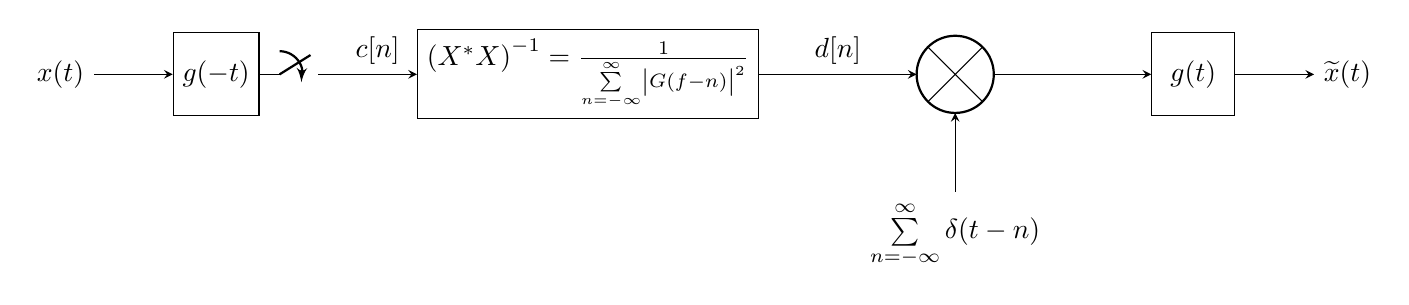
\begin{tikzpicture}[auto, node distance=2cm,]
			\node [block] (sampler) {$g(-t)$};
			\node [block, right = of sampler] (digital_filter) {$\left( X^* X \right)^{-1} = \frac{1}{\sum\limits_{n = -\infty}^{\infty} \left| G(f - n) \right|^2}$};
			\node [mixer, right = of digital_filter] (mixer) {};
			\node [block, right = of mixer] (reconstructor) {$g(t)$};

			\draw [stealth-] (sampler.west) -- ++(-1,0) node [left] {$x(t)$};
			\draw (sampler.east) to [switch] ++(1,0) [-stealth] -- (digital_filter.west) node [midway, above] {$c[n]$};
			\draw [-stealth] (digital_filter.east) -- (mixer.west) node [midway, above] {$d[n]$};
			\draw [stealth-] (mixer.south) -- ++(0,-1) node [below] {$\sum\limits_{n = -\infty}^{\infty} \delta(t - n)$};
			\draw [-stealth] (mixer.east) -- (reconstructor.west) node [right] {};
			\draw [-stealth] (reconstructor.east) -- ++(1,0) node [right] {$\tilde{x}(t)$};
		\end{tikzpicture}
		\end{adjustbox}
		\caption{Generalized Sampling and Reconstruction}
		\label{fig:generalized_sampling_and_reconstruction}
	\end{figure}
\end{theorem}

\begin{proof}
	\begin{align*}
		c_i &= \left\langle x_i , \sum\limits_{n = -\infty}^{\infty} x_n d_n \right\rangle\\
		&= \left\langle g(t - i) , \sum\limits_{n = -\infty}^{\infty} d_n g(t - n) \right\rangle\\
		&= \sum\limits_{n = -\infty}^{\infty} d_n \left\langle g(t - i) , g(t - n) \right\rangle\\
		&= \sum\limits_{n = -\infty}^{\infty} d_n \int\limits_{-\infty}^{\infty} g(t - i)^* g(t - n) \dif t
	\end{align*}
	Substituting $t' = t - i$,
	\begin{align*}
		c_i &= \sum\limits_{n = -\infty}^{\infty} d_n \int\limits_{-\infty}^{\infty} {g(t')}^* g(t' - n + i) \dif t'
	\end{align*}
	Let
	\begin{align*}
		y(t) &= g^*(t) \ast g(-t)
	\end{align*}
	Therefore,
	\begin{align*}
		c_i &= \sum\limits_{n = -\infty}^{\infty} d_n y(i - n)\\
		&= (d \ast y)[i]
	\end{align*}
	Hence,
	\begin{align*}
		c[n] &= d[i] \ast y[i]
	\end{align*}
	Therefore,
	\begin{align*}
		C\left( e^{j 2 \pi f} \right) &= D\left( e^{j 2 \pi f} \right) \DTFT\left\{ y[n] \right\}\\
		&= D\left( e^{j 2 \pi f} \right) \DTFT\left\{ g^*(t) \ast g(-t) \right\}\\
		&= D\left( e^{j 2 \pi f} \right) \sum\limits_{n = -\infty}^{\infty} G^*(f - n) G(f - n)\\
		&= D\left( e^{j 2 \pi f} \right) \sum\limits_{n = -\infty}^{\infty} \left| G(f - n) \right|^2
	\end{align*}
	Therefore,
	\begin{align*}
		D\left( e^{j 2 \pi f} \right) &= \frac{1}{\sum\limits_{n = -\infty}^{\infty} \left| G(f - n) \right|^2} C\left( e^{j 2 \pi f} \right)
	\end{align*}
\end{proof}

\begin{theorem}
	Let $X : \l2 \to H$ and $S : \l2 \to H$ be a set transformations corresponding to shift invariant functions
	\begin{align*}
		x_i &= g(t - i)
	\end{align*}
	and
	\begin{align*}
		y_i &= s(t - i)
	\end{align*}
	respectively.
	Then, if $S^* X$ is invertible, a generalized sampling and reconstruction using these basis elements can be performed as in \cref{fig:generalized_sampling_and_reconstruction_with_different_sampling_and_reconstruction_bases}.
	\begin{figure}[H]
		\centering
		\begin{adjustbox}{max width=\columnwidth}
		\begin{tikzpicture}[auto, node distance=2cm,]
			\node [block] (sampler) {$s(-t)$};
			\node [block, right = of sampler] (W) {$W = \left( S^* X \right)^{-1}$};
			\node [mixer, right = of W] (mixer) {};
			\node [block, right = of mixer] (reconstructor) {$g(t)$};

			\draw [stealth-] (sampler.west) -- ++(-1,0) node [left] {$x(t)$};
			\draw (sampler.east) to [switch] ++(1,0) [-stealth] -- (W.west) node [midway, above] {$c[n]$};
			\draw [-stealth] (W.east) -- (mixer.west) node [midway, above] {$d[n]$};
			\draw [stealth-] (mixer.south) -- ++(0,-1) node [below] {$\sum\limits_{n = -\infty}^{\infty} \delta(t - n)$};
			\draw [-stealth] (mixer.east) -- (reconstructor.west) node [right] {};
			\draw [-stealth] (reconstructor.east) -- ++(1,0) node [right] {$\tilde{x}(t)$};
		\end{tikzpicture}
		\end{adjustbox}
		\caption{Generalized Sampling and Reconstruction with Different Sampling and Reconstruction Bases}
		\label{fig:generalized_sampling_and_reconstruction_with_different_sampling_and_reconstruction_bases}
	\end{figure}
\end{theorem}

\begin{theorem}
	Let $\{s_n\}$ and $\{g_n\}$ span the Riesz bases $S$ and $X$ respectively.
	Assume
	\begin{align*}
		H &= {\range(S)}^{\perp} \cup \range(X)
	\end{align*}
	Then, $S^* X : \l2 \to \l2$ is invertible iff
	\begin{align*}
		{\range(S)}^{\perp} \cap \range(X) &= \{0\}
	\end{align*}
	Hence,
	\begin{align*}
		H &= {\range(S)}^{\perp} \oplus X
	\end{align*}
\end{theorem}

\section{Common Shift Invariant Riesz Bases}

\begin{definition}[Spline]
	A spline of order $n$ is defined as
	\begin{align*}
		x(t) &= \sum\limits_{k = -\infty}^{\infty} d_k \beta^n(t - k)
	\end{align*}
	where
	\begin{align*}
		\beta^0(t) &=
			\begin{cases}
				1 &;\quad |t| < 0.5\\
				\frac{1}{2} &;\quad |t| = 0.5\\
				0 &;\quad \text{otherwise}\\
			\end{cases}\\
		\beta^n(t) &= \beta^0(t) \ast \beta^{n - 1}(t)
	\end{align*}
	Hence, splines are a shift invariant Riesz basis.
	\index{spline}
\end{definition}

\begin{definition}[Lanczos interpolation]
	Lanczos interpolation with parameter $a$ is defined with basis elements $g(t)$ such that
	\begin{align*}
		g(t) &=
			\begin{cases}
				\sinc(t) \sinc\left( \frac{t}{a} \right) &;\quad |t| < a\\
				0 &;\quad \text{otherwise}\\
			\end{cases}
	\end{align*}
	Hence, the basis is a shift invariant Riesz basis.
	\index{Lanczos interpolation}
\end{definition}

\clearpage
\part{Resampling}

\section{Downsampling}

\begin{definition}[Downsampling operator]
	The downsampling operator $\downarrow$ is defined such that if
	\begin{align*}
		g &= \downsample{M} f
	\end{align*}
	then
	\begin{align*}
		g[n] &= f[M n]
	\end{align*}
	\index{downsampling}
\end{definition}

\begin{theorem}
	\begin{align*}
		\downsample{M} (\alpha f + \beta g) &= \alpha \downsample{M} f + \beta \downsample{M} g
	\end{align*}
	\index{downsampling}
\end{theorem}

\begin{theorem}
	\begin{align*}
		\downsample{M_1} \downsample{M_2} f &= \downsample{M_1 M_2} f
	\end{align*}
	\index{downsampling}
\end{theorem}

\begin{theorem}
	Let $D_p$ be a translation operator, i.e.
	\begin{align*}
		D_p f[n] &= f[n - p]
	\end{align*}
	Then,
	\begin{align*}
		D_p \downsample{M} f &= \downsample{M} D_{M p} f
	\end{align*}
	\index{downsampling}
\end{theorem}

\begin{theorem}
	Let $H$ be an LTI filter.
	Then,
	\begin{align*}
		H \downsample{M} &= \downsample{M} G
	\end{align*}
	where
	\begin{align*}
		G &= \sum\limits_{m = -\infty}^{\infty} h[m] D_{M m}
	\end{align*}
	with impulse response
	\begin{align*}
		g[m] &=
			\begin{cases}
				h\left[ \frac{m}{M} \right] &;\quad \frac{m}{M} \in \mathbb{Z}\\
				0 &;\quad \text{otherwise}\\
			\end{cases}
	\end{align*}
	where $h[n]$ is the impulse response of $H$.
	Also,
	\begin{align*}
		G(f) &= H(M f)
	\end{align*}
\end{theorem}

\begin{proof}
	\begin{align*}
		(H f)[n] &= (h \ast f)[n]\\
		&= \sum\limits_{m = -\infty}^{\infty} h[m] f[n - m]\\
		&= \left( \sum\limits_{m = -\infty}^{\infty} h[m] \delta[n - m] \right) \ast f[n]\\
		&= \left( \sum\limits_{m = -\infty}^{\infty} h[m] D_n \right) f[n]
	\end{align*}
	Therefore,
	\begin{align*}
		H \downsample{M} &= \sum\limits_{m = -\infty}^{\infty} h[m] (D_M \downsample{M})\\
		&= \sum\limits_{m = -\infty}^{\infty} (\downsample{M} D_{M m})\\
		&= \downsample{M} \left( \sum\limits_{m = -\infty}^{\infty} h[m] D_{M m} \right)\\
		&= \downsample{M} G
	\end{align*}
	where
	\begin{align*}
		G &= \sum\limits_{m = -\infty}^{\infty} h[m] D_{M m}
	\end{align*}
	Hence,
	\begin{align*}
		G &= \sum\limits_{m = -\infty}^{\infty} h[m] D_{M m}\\
		&= \sum\limits_{\frac{m'}{M} = -\infty}^{\infty} h\left[ \frac{m'}{M} \right] D_{m'}
	\end{align*}
	Hence,
	\begin{align*}
		g[m] &=
			\begin{cases}
				h\left[ \frac{m}{M} \right] &;\quad \frac{m}{M} \in \mathbb{Z}\\
				0 &;\quad \text{otherwise}\\
			\end{cases}
	\end{align*}
	Hence,
	\begin{align*}
		G(f) &= \sum\limits_{n = -\infty}^{\infty} g[n] e^{-2 \pi j f n}\\
		&= \sum\limits_{n = -\infty}^{\infty} h[n] e^{-2 \pi j f M n}\\
		&= H(M f)
	\end{align*}
\end{proof}

\begin{theorem}[Noble Identity for Downsampling]
	\begin{align*}
		h \ast (\downsample{M} f) &= \downsample{M} \left( (\upsample{M} h) \ast f \right)
	\end{align*}
	Equivalently, downsampling by $M$ and then applying $H(f)$ is equivalent to applying $H(f)$ and then downsampling by $M$.
	\index{Noble Identity!downsampling}
	\label{thm:Noble_identity_for_downsampling}
\end{theorem}

\section{Upsampling}

\begin{definition}[Upsampling operator]
	The upsampling operator $\uparrow$ is defined such that if
	\begin{align*}
		g &= \upsample{M} f
	\end{align*}
	then
	\begin{align*}
		g[n] &=
			\begin{cases}
				f\left[ \frac{n}{M} \right] &;\quad \frac{n}{M} \in \mathbb{Z}\\
				0 &;\quad \text{otherwise}\\
			\end{cases}
	\end{align*}
	\index{upsampling}
\end{definition}

\begin{theorem}
	\begin{align*}
		\upsample{M_1} \upsample{M_2} f &= \upsample{M_1 M_2} f
	\end{align*}
	\index{upsampling}
\end{theorem}

\begin{theorem}
	\begin{align*}
		\upsample{M} (\alpha f + \beta g) &= \alpha \upsample{M} f + \beta \upsample{M} g
	\end{align*}
	\index{upsampling}
\end{theorem}

\begin{theorem}
	Let $D_p$ be a translation operator, i.e.
	\begin{align*}
		D_p f[n] &= f[n - p]
	\end{align*}
	Then,
	\begin{align*}
		\upsample{M} D_p f &= D_{M p} \upsample{M} f
	\end{align*}
	\index{upsampling}
\end{theorem}

\begin{theorem}
	Let $H$ be an LTI filter.
	Then,
	\begin{align*}
		\upsample{M} H &= G \upsample{M}
	\end{align*}
	where
	\begin{align*}
		G &= \sum\limits_{m = -\infty}^{\infty} h[m] D_{M m}
	\end{align*}
	with impulse response
	\begin{align*}
		g[m] &=
			\begin{cases}
				h\left[ \frac{m}{M} \right] &;\quad \frac{m}{M} \in \mathbb{Z}\\
				0 &;\quad \text{otherwise}\\
			\end{cases}
	\end{align*}
	where $h[n]$ is the impulse response of $H$.
	Also,
	\begin{align*}
		G(f) &= H(M f)
	\end{align*}
\end{theorem}

\begin{theorem}[Noble Identity for Upsampling]
	\begin{align*}
		\upsample{M} (h \ast f) &= \left( \upsample{M} h \right) \ast \left( \upsample{M} f \right)
	\end{align*}
	Equivalently, applying $H(f)$ and then upsampling by $M$ is equivalent to upsampling by $M$ and then applying $H(M f)$.
	\index{Noble Identity!upsampling}
	\label{thm:Noble_identity_for_upsampling}
\end{theorem}

\section{Polyphase Representation}

\begin{theorem}[Type 1 Polyphase Decomposition]
	\begin{align*}
		\sum\limits_{n = -\infty}^{\infty} f[n] &= \sum\limits_{m = 0}^{M - 1} \sum\limits_{n = -\infty}^{\infty} f[M n + m]
	\end{align*}
	Therefore, for a linear shift invariant system
	\begin{align*}
		H &= \sum\limits_{n = -\infty}^{\infty} h[n] D_n
	\end{align*}
	the polyphase component of $h[n]$ with respect to $M$ can be defined as
	\begin{align*}
		e_m[n] &= h[M n + m]
	\end{align*}
	Hence,
	\begin{align*}
		(h \ast f)[n] &= \sum\limits_{m = 0}^{M - 1} (\upsample{M} e_m) \ast f[n - m]
	\end{align*}
	and equivalently,
	\begin{align*}
		H(f) &= \sum\limits_{m = 0}^{M - 1} E_m(M f) e^{-2 \pi j f n}
	\end{align*}
	where
	\begin{align*}
		E_m &= \FT\left\{ e_m \right\}
	\end{align*}
	\index{polyphase decomposition!type 1}
	\label{thm:type_1_polyphase_decomposition}
\end{theorem}

\begin{proof}
	Let $\varepsilon_m$ be a system with impulse response $e_m[n]$.
	Therefore,
	\begin{align*}
		\varepsilon_m &= \sum\limits_{n = -\infty}^{\infty} e_m[n] D_n\\
		&= \sum\limits_{n = -\infty}^{\infty} h[M n + m]
	\end{align*}
	Therefore,
	\begin{align*}
		H &= \sum\limits_{m = -}^{M - 1} \sum\limits_{n = -\infty}^{\infty} h[M n + m] D_{M n + m}\\
		&= \sum\limits_{m = 0}^{M - 1} \left( \sum\limits_{n = -\infty}^{\infty} h[M n + m] D_{M n} \right) D_m\\
		&= \sum\limits_{m = 0}^{M - 1} \left( \sum\limits_{n = -\infty}^{\infty} e_m[n] D_{M n} \right) D_m
	\end{align*}
	Therefore,
	\begin{align*}
		(h \ast f)[n] &= \sum\limits_{m = 0}^{M - 1} (\upsample{M} e_m) \ast f[n - m]
	\end{align*}
	and equivalently,
	\begin{align*}
		H(f) &= \sum\limits_{m = 0}^{M - 1} E_m(M f) e^{-2 \pi j f m}
	\end{align*}
	where
	\begin{align*}
		E_m &= \FT\left\{ e_m \right\}
	\end{align*}
\end{proof}

\begin{theorem}[Type 2 Polyphase Decomposition]
	\begin{align*}
		\sum\limits_{n = -\infty}^{\infty} f[n] &= \sum\limits_{m = 0}^{M - 1} \sum\limits_{n = -\infty}^{\infty} f[M n + m]
	\end{align*}
	Therefore, for a linear shift invariant system
	\begin{align*}
		H &= \sum\limits_{n = -\infty}^{\infty} h[n] D_n
	\end{align*}
	the polyphase component of $h[n]$ with respect to $M$ can be defined as
	\begin{align*}
		r_m[n] &= h[M n - m]
	\end{align*}
	Hence,
	\begin{align*}
		(h \ast f)[n] &= \sum\limits_{m = 0}^{M - 1} \left( \left( \upsample{M} r_m \right) \ast f \right) [n + m]
	\end{align*}
	and equivalently,
	\begin{align*}
		H(f) &= \sum\limits_{m = 0}^{M - 1} R_m(M f) e^{-j 2 \pi f (M - 1 - m)}
	\end{align*}
	where
	\begin{align*}
		R_m &= \FT\left\{ r_m \right\}
	\end{align*}
	\index{polyphase decomposition!type 2}
	\label{thm:type_2_polyphase_decomposition}
\end{theorem}

\begin{proof}
	Let $\varepsilon_m$ be a system with impulse response $e_m[n]$.
	Therefore,
	\begin{align*}
		\varepsilon_m &= \sum\limits_{n = -\infty}^{\infty} e_m[n] D_n\\
		&= \sum\limits_{n = -\infty}^{\infty} h[M n + m]
	\end{align*}
	Therefore,
	\begin{align*}
		H &= \sum\limits_{m = -}^{M - 1} \sum\limits_{n = -\infty}^{\infty} h[M n + m] D_{M n + m}\\
		&= \sum\limits_{m = 0}^{M - 1} \left( \sum\limits_{n = -\infty}^{\infty} h[M n + m] D_{M n} \right) D_m\\
		&= \sum\limits_{m = 0}^{M - 1} \left( \sum\limits_{n = -\infty}^{\infty} e_m[n] D_{M n} \right) D_m
	\end{align*}
	Therefore,
	\begin{align*}
		(h \ast f)[n] &= \sum\limits_{m = 0}^{M - 1} (\upsample{M} e_m) \ast f[n - m]
	\end{align*}
	and equivalently,
	\begin{align*}
		H(f) &= \sum\limits_{m = 0}^{M - 1} E_m(M f) e^{-2 \pi j f m}
	\end{align*}
	where
	\begin{align*}
		E_m &= \FT\left\{ e_m \right\}
	\end{align*}
	Let
	\begin{align*}
		r_m[n] &= e_{-m}[n]\\
		&= h[M n - m]
	\end{align*}
	Therefore,
	\begin{align*}
		H &= \sum\limits_{m = 0}^{M - 1} D_{-m} \left( \sum\limits_{n = -\infty}^{\infty} r_m[n] D_{M n} \right)\\
		&= \sum\limits_{m = 0}^{M - 1} D_{-m} \left( \sum\limits_{n = -\infty}^{\infty} \left( \upsample{M} r_m \right)[n] D_n \right)
	\end{align*}
	Therefore,
	\begin{align*}
		(h \ast f)[n] &= \sum\limits_{m = 0}^{M - 1} \left( \left( \upsample{M} r_m \right) \ast f \right)[n + m]
	\end{align*}
\end{proof}

\section{Efficient Implementation of Decimators}

\begin{theorem}
	Let $H$ be a linear shift invariant system with impulse response $h[n]$, and polyphase component
	\begin{align*}
		e_m[n] &= h[M n - m]
	\end{align*}
	Then,
	\begin{align*}
		\downsample{M} H &= \sum\limits_{m = 0}^{M - 1} \varepsilon_m \downsample{M} D_m
	\end{align*}
	where $\varepsilon_m$ is the system with impulse response $e_m[n]$.\\
	Therefore, for a signal $x \in \mathbb{R}^{N^d}$ and a filter $h \in \mathbb{R}^{k^d}$, the cost of applying the LHS is $\O\left( N^d k^d \right)$, while the cost of applying the RHS is $\O\left( \frac{N^d k^d}{M^d} \right)$, i.e. the RHS is more efficient by a factor of $M^d$.
\end{theorem}

\begin{proof}
	\begin{align*}
		\downsample{M} H f &= \sum\limits_{m = 0}^{M - 1} \upsample{M} \varepsilon_m \ast D_m f\\
	\end{align*}
	Therefore, by \cref{thm:Noble_identity_for_downsampling},
	\begin{align*}
		\downsample{M} H f &= \sum\limits_{m = 0}^{M - 1} e_m \ast \downsample{M} D_m f\\
		&= \sum\limits_{m = 0}^{M - 1} \varepsilon_m \downsample{M} D_m f
	\end{align*}
	Hence,
	\begin{align*}
		\downsample{M} H &= \sum\limits_{m = 0}^{M - 1} \varepsilon_m \downsample{M} D_m
	\end{align*}
\end{proof}

\section{Efficient Implementation of Interpolation}

\begin{theorem}
	Let $H$ be a linear shift invariant system with impulse response $h[n]$, and polyphase component
	\begin{align*}
		e_m[n] &= h[M n - m]
	\end{align*}
	Then,
	\begin{align*}
		H \upsample{M} &= \sum\limits_{m = 0}^{M - 1} D_{-m} \upsample{M} \mathcal{R}_m
	\end{align*}
	where $\mathcal{R}_m$ is the system with impulse response $r_m[n]$.\\
\end{theorem}

\begin{proof}
	\begin{align*}
		H \upsample{M} f &= \sum\limits_{m = 0}^{M - 1} D_{-m} \left( \upsample{M} r_m \ast \upsample{M} f \right)
	\end{align*}
	Therefore, by \cref{thm:Noble_identity_for_upsampling},
	\begin{align*}
		H \upsample{M} f &= \sum\limits_{m = 0}^{M - 1} D_{-m} \upsample{M} r_m \ast f\\
		&= \sum\limits_{m = 0}^{M - 1} D_{-m} \upsample{M} \mathcal{R}_m f
	\end{align*}
	Hence,
	\begin{align*}
		H \upsample{M} &= \sum\limits_{m = 0}^{M - 1} D_{-m} \upsample{M} \mathcal{R}_m
	\end{align*}
\end{proof}

\clearpage
\part{Short Time Fourier Transform}

\section{Short Time Fourier Transform}

\begin{definition}[Short time Fourier transform]
	The short time Fourier transform of a signal $f(t)$ is defined to be
	\begin{align*}
		\hat{x}(f,\tau) &= \int\limits_{-\infty}^{\infty} x(t) w(t - \tau) e^{-j 2 \pi f t} \dif t
	\end{align*}
	where $w(t)$ is the window function.\\
	Equivalently,
	\begin{align*}
		x(t) w(t - \tau) &= \int\limits_{-\infty}^{\infty} \hat{x}(f,\tau) e^{j 2 \pi f t} \dif f
	\end{align*}
	This allows for localization in the time domain which is not possible when using Fourier transform.
	\index{transform!Fourier!short time}
\end{definition}

\begin{definition}[Gabor transform]
	The short time Fourier transform with window function
	\begin{align*}
		w(t) &= e^{-\frac{t^2}{\sigma^2}}
	\end{align*}
	is called the Gabor transform.
	\index{transform!Gabor}
\end{definition}

\section{Inverse Short Time Fourier Transform}

\begin{theorem}
	\begin{align*}
		x(t) &= \IFT\left\{ \int\limits_{-\infty}^{\infty} x(f,\tau) \dif \tau \right\}
	\end{align*}
	\index{transform!Fourier!short time}
\end{theorem}

\begin{proof}
	Let $w(t)$ be a window function such that
	\begin{align*}
		\int\limits_{-\infty}^{\infty} w(t) \dif t &= 1
	\end{align*}
	Therefore, for any $\tau \in \mathbb{R}$,
	\begin{align*}
		\int\limits_{-\infty}^{\infty} w(t - \tau) \dif t &= 1\\
		\int\limits_{-\infty}^{\infty} w(t - \tau) \dif \tau &= 1
	\end{align*}
	Therefore,
	\begin{align*}
		\int\limits_{-\infty}^{\infty} \hat{x}(f,\tau) \dif \tau &= \int\limits_{-\infty}^{\infty} \int\limits_{-\infty}^{\infty} x(t) w(t - \tau) e^{-j 2 \pi f t} \dif t \dif \tau\\
		&= \int\limits_{-\infty}^{\infty} x(t) e^{-j 2 \pi f t} \left( \int\limits_{-\infty}^{\infty} w(t - \tau) \dif \tau \right) \dif t\\
		&= \int\limits_{-\infty}^{\infty} x(t) e^{-j 2 \pi f t} (1) \dif t\\
		&= X(f)
	\end{align*}
	Therefore,
	\begin{align*}
		x(t) &= \IFT\left\{ \int\limits_{-\infty}^{\infty} x(f,\tau) \dif \tau \right\}
	\end{align*}
\end{proof}

\begin{theorem}
	\begin{align*}
		\IFT\left\{ x(t,\tau) \right\} &= x(t) w(t - \tau)
	\end{align*}
	\index{transform!Fourier!short time}
\end{theorem}

\begin{proof}
	\begin{align*}
		x(t) &= \int\limits_{-\infty}^{\infty} \int\limits_{-\infty}^{\infty} x(f,\tau) e^{2 \pi f t} \dif \tau \dif f\\
		&= \int\limits_{-\infty}^{\infty} \left( \int\limits_{-\infty}^{\infty} x(f,\tau) e^{j 2 \pi f t} \dif f \right) \dif \tau
	\end{align*}
	Also,
	\begin{align*}
		x(t) &= \int\limits_{-\infty}^{\infty} x(t) w(t - \tau) \dif \tau
	\end{align*}
	Therefore,
	\begin{align*}
		\IFT\left\{ x(t,\tau) \right\} &= x(t) w(t - \tau)
	\end{align*}
\end{proof}

\section{Discrete Short Time Fourier Transform}

\begin{theorem}
	Assume constant overlap-add (COLA) for hop size $R$, i.e.
	\begin{align*}
		\sum\limits_{m = -\infty}^{\infty} w(n - m R) &= 1
	\end{align*}
	Then,
	\begin{align*}
		x(n) &= \IDTFT\left\{ \sum\limits_{m = -\infty}^{\infty} X_m(f) \right\}
	\end{align*}
	where
	\begin{align*}
		X_m(f) &= \DTFT\left\{ x(t) D_{m R}\left( w(t) \right) \right\}
	\end{align*}
\end{theorem}

\begin{proof}
	For simplicity, assume that the sampling is performed with $T = 1$.
	Hence, let
	\begin{align*}
		X_m(f) &= \DTFT\left\{ x(t) D_{m R}\left( w(t) \right) \right\}\\
		&= \sum\limits_{n = -\infty}^{\infty} x(n) w(n - m R) e^{-j 2 \pi f n}
	\end{align*}
	where
	\begin{align*}
		D_{m R}(w) &= w(n - m R)
	\end{align*}
	and $R$ is called the hop size.\\
	Assume constant overlap-add (COLA) for hop size $R$, i.e.
	\begin{align*}
		\sum\limits_{m = -\infty}^{\infty} w(n - m R) &= 1
	\end{align*}
	Therefore,
	\begin{align*}
		\sum\limits_{m = -\infty}^{\infty} X_m(f) &= \sum\limits_{m = -\infty}^{\infty} \sum\limits_{n = -\infty}^{\infty} x(n) w(n - m R) e^{-j 2 \pi f n}\\
		&= \sum\limits_{n = -\infty}^{\infty} x(n) e^{-j 2 \pi f n} \sum\limits_{m = -\infty}^{\infty} w(n - m R)\\
		&= \sum\limits_{n = -\infty}^{\infty} x(n) e^{-j 2 \pi f n} (1)\\
		&= \DTFT\left\{ x(n) \right\}
	\end{align*}
	Therefore,
	\begin{align*}
		x(n) &= \IDTFT\left\{ \sum\limits_{m = -\infty}^{\infty} X_m(f) \right\}
	\end{align*}
\end{proof}

\subsection{Discrete STFT using Fast Fourier Transform}

\begin{definition}[Discrete short time Fourier transform using FFT]
	Let
	\begin{align*}
		\tilde{x_m(n)} &= x(n + m R)
	\end{align*}
	for $n \in \mathbb{Z}$, and $-M \le n \le M$, where $M$ is called the frame length.
	Then,
	\begin{align*}
		X_m(f) &= \FT\left\{ x_m(t) \right\}\\
		&= e^{-j 2 \pi f m R} \DTFT\left\{ D_{-m R}\left( x(t) \right) w(t) \right\}\\
		&= e^{-j 2 \pi f m R} \DTFT\left\{ \tilde{x_m}(n) w(n) \right\}
	\end{align*}
	Hence, let
	\begin{align*}
		\tilde{x_m}^{w}(n) &=
			\begin{cases}
				\tilde{x_m}(n) w(n) &;\quad |n| \le M\\
				0 &;\quad M < n \le \frac{N}{2} - 1\\
				0 &;\quad -\frac{N}{2} \le n < -M\\
			\end{cases}
	\end{align*}
	Then,
	\begin{align*}
		\FFT_{k}\left\{ \tilde{x_m}^{w}(n) \right\} &= e^{-j 2 \pi \frac{k}{N} m R} \FFT\left\{ \tilde{x_m}^w(n) \right\}
	\end{align*}
	is called the time normalized STFT, where $k$ is called the bin number, and $m$ is called the frame number, $N$ is the size of the FFT, and $M_w = 2 M + 1$ is the size of the filter $w(n)$.
	\index{transform!Fourier!discrete short time!using FFT}
\end{definition}

\subsection{Discrete STFT using Filter Bank Summation Interpolation}

\begin{definition}[Discrete short time Fourier transform using filter banks]
	\begin{align*}
		x_m(k) &= \sum\limits_{n = -\infty}^{\infty} x(n) e^{-j 2 \pi \frac{k}{N} n} w(n - m R)
	\end{align*}
	Hence, let
	\begin{align*}
		x_k(n) &= x(n) e^{-j 2 \pi \frac{k}{N} n}
	\end{align*}
	Therefore,
	\begin{align*}
		x_m(k) &= x_k(m R) \ast w(-m R)
	\end{align*}
	Hence, $x_m(k)$ can be obtained by passing $x(n)$ through a filter bank as in \cref{fig:discrete_STFT_implementation_using_filter_banks}.
	\begin{figure}[H]
		\centering
		\begin{adjustbox}{max width=\columnwidth}
		\begin{tikzpicture}[auto, node distance=2cm,]
			\node [mixer] (mixer1) at (0,2) {};
			\node [mixer] (mixern) at (0,-2) {};
			\node at (0,0) {$\vdots$};

			\node [block, right = of mixer1] (filter1) {$w[-n]$};
			\node [block, right = of mixern] (filtern) {$w[-n]$};

			\node [block, right = of filter1] (downsampler1) {$\downsample{R}$};
			\node [block, right = of filtern] (downsamplern) {$\downsample{R}$};

			\draw [-stealth] (-2,0) node [left] {$x[n]$} -| (-1,2) -- (mixer1.west);
			\draw [-stealth] (-2,0) node [left] {$x[n]$} -| (-1,-2) -- (mixern.west);

			\draw [-stealth] (mixer1.east) -- (filter1.west);
			\draw [-stealth] (mixern.east) -- (filtern.west);

			\draw [-stealth] (filter1.east) -- (downsampler1.west);
			\draw [-stealth] (filtern.east) -- (downsamplern.west);

			\draw [-stealth] (downsampler1.east) -- ++(1,0) node [right] {$x_m(0)$};
			\draw [-stealth] (downsamplern.east) -- ++(1,0) node [right] {$x_m(n - 1)$};

			\draw [stealth-] (mixer1.north) -- ++(0,1) node [above] {$e^{-j 2 \pi \frac{0}{N} n}$};
			\draw [stealth-] (mixern.south) -- ++(0,-1) node [below] {$e^{-j 2 \pi \frac{N - 1}{N} n}$};
		\end{tikzpicture}
		\end{adjustbox}
		\caption{Discrete STFT Implementation using Filter Banks}
		\label{fig:discrete_STFT_implementation_using_filter_banks}
	\end{figure}
	\index{transform!Fourier!discrete short time!using filter banks}
\end{definition}

\clearpage
\part{Wavelets}

\begin{definition}[Orthogonal wavelets]
	Let $\psi: \mathbb{R} \to \mathbb{C}$, and
	\begin{align*}
		\psi_{n,k}(t) &= 2^{\frac{n}{2}} \psi\left( 2^n t - k \right)
	\end{align*}
	where $n, k \in \mathbb{Z}$.
	Such a family of $\psi_{n,k}$, which is orthonormal, and
	\begin{align*}
		L_2 &= {\vspan{\left\{ \psi_{n,k} \right\}}}^{C}
	\end{align*}
	is called a family of orthonormal wavelets, and $\psi$ called the mother wavelet.
	\index{wavelet!orthogonal}
	\index{wavelet!mother}
\end{definition}
%
\section{The Haar Wavelet}

\begin{definition}
	The family of wavelets defined by the mother wavelet
	\begin{align*}
		\psi(t) &= u_{\left[ 0, \frac{1}{2} \right]}(t) - u_{\left[ \frac{1}{2},1 \right]}(t)
	\end{align*}
	and
	\begin{align*}
		\psi_{n,k}(t) &= 2^{\frac{n}{2}} \psi\left( 2^n t - k \right)\\
		&= 2^{\frac{n}{2}} \left( u_{\left[ \frac{k}{2^n} , \frac{k + \frac{1}{2}}{2^n} \right]} - u_{\left[ \frac{k + \frac{1}{2}}{2^n} , \frac{k + 1}{2^n} \right]} \right)
	\end{align*}
	is called the family of Haar wavelets.
	\index{wavelet!Haar}
\end{definition}

\begin{theorem}
	The set of Haar wavelets $\left\{ \psi_{i,k} \right\}$ is orthonormal.
	\index{wavelet!Haar}
\end{theorem}

\begin{theorem}
	For Haar wavelets,
	\begin{align*}
		u_{[0,1]}(t) &= \sum\limits_{i < 0} 2^{\frac{i}{2}} \psi_{i,0}(t)
	\end{align*}
	\index{wavelet!Haar}
\end{theorem}

\clearpage
\printindex

\end{document}
